\begin{frame}
	\frametitle*{Inhalt}
	\tableofcontents
\end{frame}

\section{Aufgabe}
\begin{frame}
	\frametitle*{Aufgabe}
	\begin{itemize}
		\item Erstellung eines REST-Webservices
		\begin{itemize}
			\item Implementierung in PHP mit Slim
			\item Authentifizierung durch OAuth2
			\item Verschlüsslung durch HTTPS
		\end{itemize}
		\item Erstellung einer Webanwendung als Client
		\item Szenario: Bikesharing
	\end{itemize}
\end{frame}

\section{Vorgehen}
\begin{frame}
	\frametitle*{Vorgehen}
	\begin{itemize}
		\item public API implementiert
		\item Client (Webanwendung) implementiert
		\item OAuth2 Server implementiert
		\item protected APIs implementiert
		\item Client-Anwendung vervollständigt
		\item Bugfixes
	\end{itemize}
\end{frame}

\section{Funktionen des Webservice}
\begin{frame}
	\frametitle*{Funktionen des Webservice}
		\begin{tabularx}{\columnwidth}{|X|p{1cm}|p{2.5cm}|p{1.5cm}|}
		\hline
		Name & Method & URL & Access \\
		\hline
		\hline
		Alle verfügbare Fahrradstationen & GET & /stations & public \\
		\hline
		Spezielle Station & GET & /stations/stationID & public \\
		\hline
		Alle verfügbaren Fahrräder & GET & /bikes & public \\
		\hline
		Spezielles Fahrrad & GET & /bikes/bikesID & public \\
		\hline
		Alle Fahrradmodelle & GET & /models & public \\
		\hline
		Spezielles Fahrradmodell & GET & /models/modelID & public \\
		\hline
		Alle Buchungen & GET & /bookings & protected \\
		\hline
		Buchung erstellen & POST & /bookings & protected \\
		\hline
		Einzelne Buchung & GET & /bookings/bookingID & protected \\
		\hline
		Einzelne Buchung stornieren & DELETE & /bookings/bookingID & protected \\
		\hline
		Einzelne Buchung bearbeiten & PUT & /bookings/bookingID & protected \\
		\hline
		Accountinformationen & GET & /account & protected \\
		\hline
	\end{tabularx}
\end{frame}

\section{Webclient}
\begin{frame}
	\frametitle*{Webclient}
	\begin{itemize}
		\item erst funktional, dann schön
		\item Nutzung von Bibliotheken (jQuery, OpenLayers)
		\item Gerüst mit PHP und HTML erstellt, Inhalt mit Javascript gefüllt
	\end{itemize}
	\begin{figure}
		\centering
		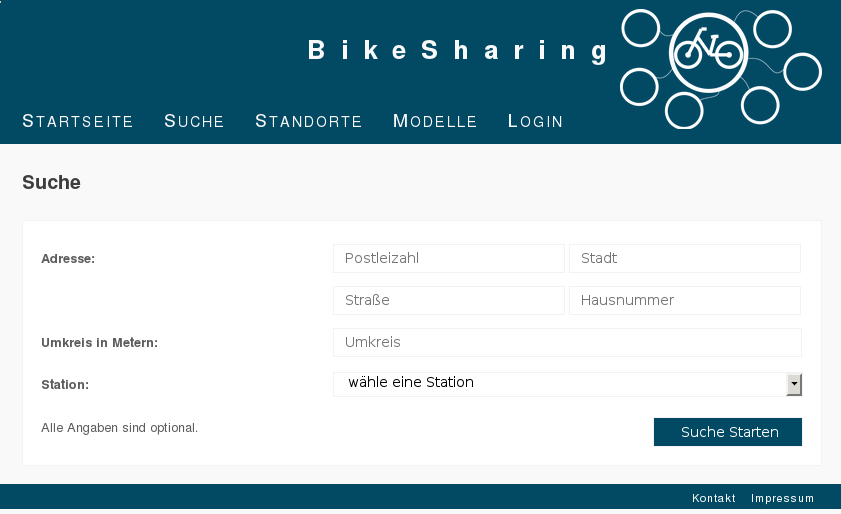
\includegraphics[height=40mm]{pics/bikesharing_search.png}
	\end{figure}
\end{frame}

\section{Implementierung des OAuth2-Servers}
\begin{frame}
	\frametitle*{Implementierung des OAuth2-Servers}
	\begin{itemize}
		\item Verwendung der \glqq OAuth2 Server Library for PHP\grqq
	\end{itemize}
	\begin{figure}
		\centering
		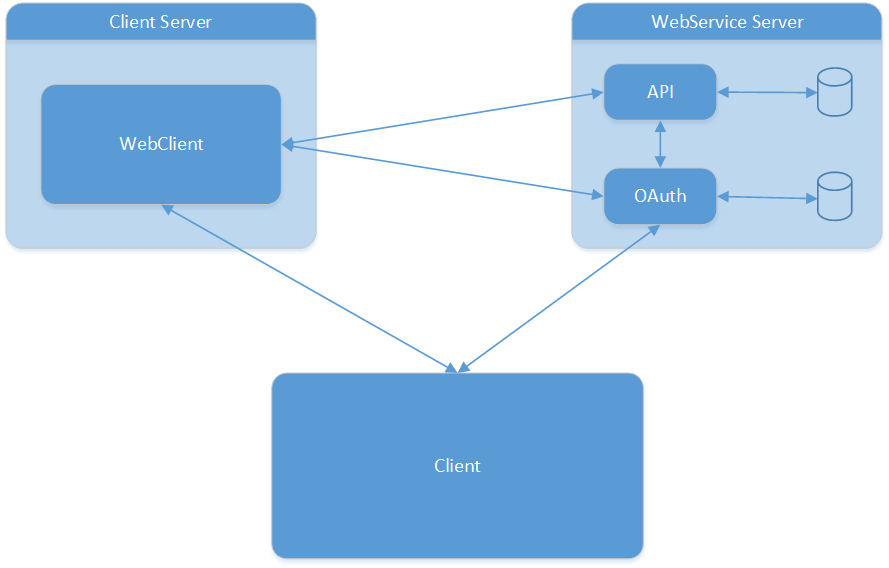
\includegraphics[height=40mm]{pics/Architektur.png}
	\end{figure}
\end{frame}

\section{Client-Anwendung}
\begin{frame}
	\frametitle*{Client-Anwendung}
	Demo
\end{frame}

\section{Fazit}
\begin{frame}
	\frametitle*{Fazit}
	\begin{itemize}
		\item Implementierung des Webclient nach Vorlage einer durchdachten API gut machbar
		\item Das Slim-Framework war eine gute Wahl, da die Verwendung sehr einfach und fehlerfrei verlief
		\begin{itemize}
			\item OAuth-Middleware hat leider nicht funktioniert
		\end{itemize}
		\item Implementierung eines OAuth-Servers ist relativ kompliziert
	\end{itemize}
\end{frame}


\section{Quellen}
\begin{frame}
	\frametitle*{Quellen}
	\begin{itemize}
		\item \url{slimframework.com}
		\item \url{jquery.com}
		\item \url{openlayers.org}
		\item \url{https://github.com/bshaffer/oauth2-server-php}
	\end{itemize}
	%\bibliography{../literatur}
\end{frame}
